\documentclass[aspectratio=169]{beamer}

\usepackage{style}
\addbibresource{references.bib}
\title[Title]{Kwantowa przewaga w grze CHSH}
\subtitle{OSSM 2026}

% \subtitle{Subtitle}

\author{Andrzej Antoni Kwaśniewski}
\date[]{10 IV 2026}
\begin{document}
% Definiowanie stopki
\onehalfspacing

%---------------------------------------------------------
\mysimplefootline
\frame{\titlepage}

%---------------------------------------------------------
\section{Section 1}
\begin{frame}{Paradoks Einsteina, Podolsky'ego, Rosena (1935)}
Mamy dwie cząstki A i B, które oddziałują a potem zostają oddalone od siebie
\begin{itemize}
    \item Mierzymy stan najpierw cząstki A, potem B
    \item Wynik pomiaru cząstki B jest znany przed pomiarem (wnioskujemy go z A)
    \item Ale B jest daleko -- pomiar A nie mógł na nią wpłynąć
    \item Zatem zdaniem EPR wynik musiał z góry ustalony - istnieją \textit{ukryte zmienne}
\end{itemize}

\vspace{0.3em}
\pause
Wniosek EPR: Albo mechanika kwantowa jest niekompletna, albo informacja rozchodzi się
szybciej niż światło.

\end{frame}

\begin{frame}{,,Bóg nie gra w kości''}

Einstein do końca życia wierzył w lokalne zmienne ukryte --
że przyroda jest deterministyczna, a losowość w mechanice kwantowej
to tylko wyraz naszej niewiedzy.

\vspace{0.3em}
\pause
\begin{theorem}{Twierdzenie Bella (1964)}
       Jeśli istnieją ukryte zmienne to korelacje między cząstkami są ograniczone
\end{theorem}
\pause
\begin{theorem}{Nierówność CHSH ( Clauser, Horne,  Shimony, Holt 1969)}
\[
|E(a,b) + E(a,b') + E(a',b) - E(a',b')| \leq 2
\]
\end{theorem}

\end{frame}
\begin{frame}{Gra CHSH}
    \begin{figure}
        \centering
        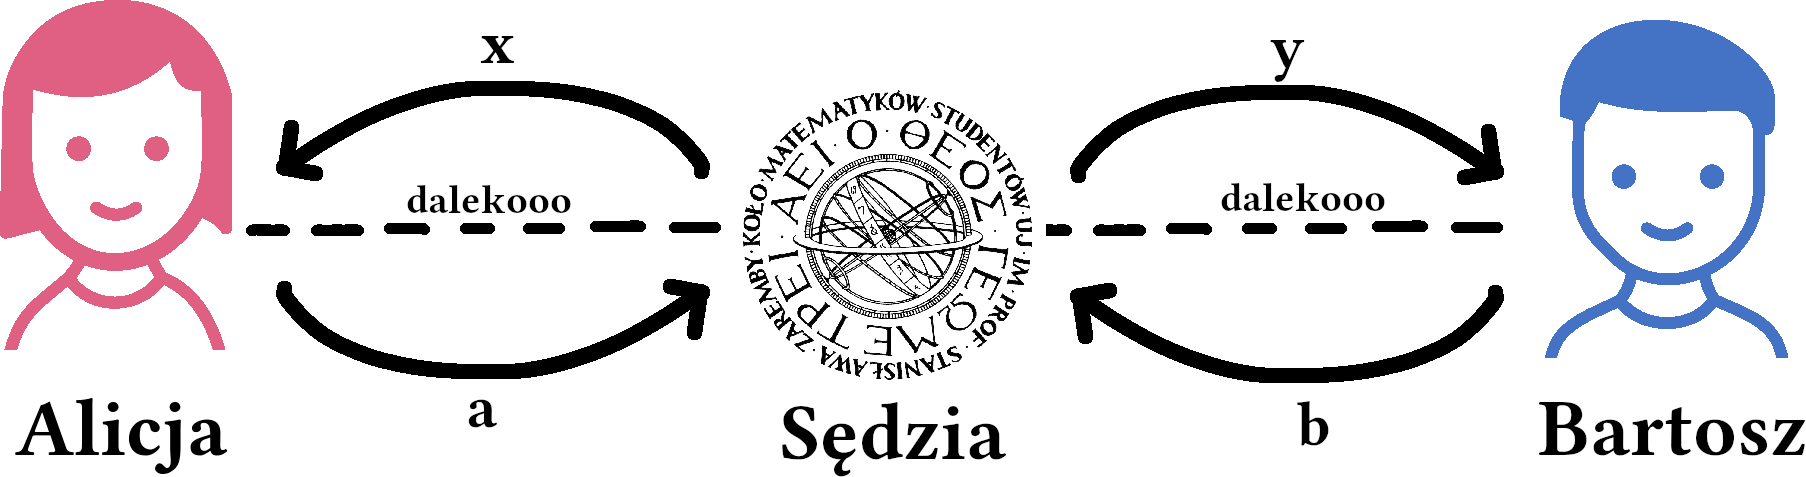
\includegraphics[width=0.65\linewidth]{images/chsh.png}
        \label{fig:enter-label}
    \end{figure}
    \begin{itemize}
        \item Sędzia losowo wybiera bity \(x\) \(y\)
        \item Wysyła bit \(x\) Alicji, bit \(y\) Bartoszowi
        \item Celem pary jest wysłanie sędziowi z powrotem takich bitów \(a\) i \(b\) aby
        \vspace{-1em}
        \[x\cdot y = a +b \mod{2}\]
        \vspace{-3em}
        \pause
        \item Gracze mogą ustalić strategię, ale NIE mogą się komunikować
    \end{itemize}
\end{frame}

\section{Section 2}
\begin{frame}{Strategia deterministyczna}
    Gracze mogą ustalić strategię. Ich strategia to para funkcji 
    \[f,g:\set{0,1} \to \set{0,1}\]
    Alicja używa funkcji \(f\), Bartosz funkcji \(g\) zatem:
    \[f(x)=a \qquad \quad g(y)=b\]
    Warunek końcowy to:
    \[x\cdot y=f(x)+g(y) \mod{2}\]
\end{frame}
\begin{frame}{Optymalna strategia deterministyczna}
    Warunek końcowy to:
    \[x\cdot y=f(x)+g(y) \mod{2}\]
    Mamy 4 możliwe wejścia
\only<1>{
\begin{align*}
    (0,0): \qquad f(0)+g(0)=0\\
    (0,1): \qquad f(0)+g(1)=0\\
    (1,0): \qquad f(1)+g(0)=0\\
    (1,1): \qquad f(1)+g(1)=1
\end{align*}
}
\only<2>{
\[
\begin{array}{rcl}
(0,0): & f(0)+g(0)=0 & \\
(0,1): & f(0)+g(1)=0 & \\
(1,0): & f(1)+g(0)=0 & \\
(1,1): & f(1)+g(1)=1 & \\
\end{array}
\;\left.\vphantom{\begin{array}{c}
(0,0)\\(0,1)\\(1,0)\\(1,1)
\end{array}}\right|\;
\begin{array}{c}
\\
\displaystyle +\\
\\
\end{array}
\]
}
\onslide<2>{
\[2[f(0)+f(1)+g(0)+g(1)]=1\]
}
\end{frame}



\section{Section 3}
\begin{frame}{Stan kubitu}

Stan kubitu opisujemy jako wektor w $\mathbb{C}^2$

\[
\ket{\psi}=
\begin{pmatrix}
\psi_1\\
\psi_2
\end{pmatrix}
\]

Warunek normalizacji:

\[
\braket{\psi|\psi}=|\psi_1|^2+|\psi_2|^2=1
\]


Możemy wybrać bazę przestrzeni $\mathbb{C}^2$

\[
\ket{0}=
\begin{pmatrix}
1\\0
\end{pmatrix},
\qquad
\ket{1}=
\begin{pmatrix}
0\\1
\end{pmatrix}
\]
\[\ket{\psi}=a \ket{0} + b \ket{1}\] 
\end{frame}

%================================================


\begin{frame}{Pomiar}
    Mierząc stan \(\ket{\psi}=a \ket{0} + b \ket{1}\) w bazie \(\ket{0}\), \(\ket{1}\)):\\
    \[P(\ket{0})=\braket{0 | \Psi}^2=\left[\begin{pmatrix}
        1 & 0
    \end{pmatrix} \begin{pmatrix}
        a \\ b 
    \end{pmatrix}\right]^2=|a|^2\]

        \[P(\ket{1})=\braket{1 | \Psi}^2=\left[\begin{pmatrix}
        0 & 1
    \end{pmatrix} \begin{pmatrix}
        a \\ b 
    \end{pmatrix}\right]^2=|b|^2\]
    \begin{tikzpicture}[remember picture,overlay]
        \node[anchor=south east, xshift=-0.2cm, yshift=0.2cm] at (current page.south east)
        {
\includegraphics[width=2cm]{images/kotek.png}};
    \end{tikzpicture}
\end{frame}


\begin{frame}{Dowolna baza}
        Dowolną bazę możemy zapisać przy pomocy bazy \(\ket{0}\) \({\ket{1}}\) jako
    \[\ket{\alpha}=\cos \theta \ket{0} + \sin \theta \ket{1}  \qquad \ket{\alpha^\perp}=-\sin \theta\ket{0} + \cos \theta\ket{1} \]
    Wtedy
    \pause
        \[P(\ket{\alpha})=\braket{\alpha | \Psi}^2=\left[\begin{pmatrix}
        \cos \theta & \sin \theta
    \end{pmatrix} \begin{pmatrix}
        a \\ b 
    \end{pmatrix}\right]^2=(a\cos \theta + b\sin \theta)^2\]
\end{frame}

%================================================


\begin{frame}{Iloczyn tensorowy}
Iloczyn tensorowy definiuje wspólny stan dwóch kubitów
\[
\ket{\psi_1} = \begin{pmatrix} a \\ b \end{pmatrix} = a\ket{0} + b\ket{1}, \quad
\ket{\psi_2} = \begin{pmatrix} c \\ d \end{pmatrix} = c\ket{0} + d\ket{1}
\]
\[
\ket{\psi_1 \psi_2}=\ket{\psi_1} \otimes \ket{\psi_2} =
\begin{pmatrix} a \\ b \end{pmatrix} \otimes 
\begin{pmatrix} c \\ d \end{pmatrix} =
\begin{pmatrix}
a \begin{pmatrix}
    c \\ d
\end{pmatrix}\\b \begin{pmatrix}
    c \\ d
\end{pmatrix}
\end{pmatrix}
=
\begin{pmatrix}
a c \\ a d \\ b c \\ b d
\end{pmatrix}
\]

\end{frame}


%================================================


\begin{frame}{Splątanie kwantowe}

Dwa kubity są splątane, jeśli ich wspólnego stanu nie da się zapisać jako
iloczynu tensorowego stanów pojedynczych kubitów:
\[
|\psi\rangle \neq |\psi_A\rangle \otimes |\psi_B\rangle
\]
\pause
Przykład stanu splątanego (stan Bella):
\vspace{-2em}
\[
|\Psi\rangle = \frac{|00\rangle + |11\rangle}{\sqrt{2}}=\begin{pmatrix}
    1 \\0 \\0 \\1
\end{pmatrix}
\]
\vspace{-2em}

Jeśli zmierzymy pierwszy kubit w bazie $|0\rangle, |1\rangle$:

\begin{itemize}
\item wynik $0$ $\Rightarrow$ drugi kubit także $0$
\item wynik $1$ $\Rightarrow$ drugi kubit także $1$
\end{itemize}

\end{frame}

%================================================


\section{Section 4}
\begin{frame}{Kwantowa strategia}
W kwantowej strategii uzyskamy prawdopodobieństwo wygranej \(\approx 0.85 > 0.75\).\\
Strategia zakłada, że Alicja i Bartosz dzielą dwukubitowy splątany stan
\[\ket{\Psi}=\frac{\ket{00}+\ket{{11}}}{\sqrt{2}}=\frac{1}{\sqrt{2}}\begin{pmatrix}
    1 \\0 \\0 \\1
\end{pmatrix}\]
 Alicji dajemy pierwszy kubit, Bartoszowi drugi.\\
 W zależności od wejścia dokonają innego pomiaru na swoim kubicie
\end{frame}


% ===================================================================


\begin{frame}{}
    Alicja robi pomiar w bazie \(\ket{\alpha}\), \(\ket{\alpha^\perp}\)
    \vspace{-0.7em}
    \[\ket{\alpha}=\cos \theta_A \ket{0} + \sin \theta_A \ket{1}  \qquad \ket{\alpha^\perp}=-\sin \theta_A \ket{0} + \cos \theta_A \ket{1} \]
    Analogicznie Bob robi pomiar w bazie \(\ket{\beta}\), \(\ket{\beta^\perp}\).
    \vspace{-0.7em}
    \[\ket{\beta}=\cos \theta_B \ket{0} + \sin \theta_B \ket{1}  \qquad \ket{\beta^\perp}=-\sin \theta_B \ket{0} + \cos \theta_B \ket{1} \]
    Zatem
    \vspace{-3em}
    \begin{align*}
\sqrt{P(a=0, b=0)}=\braket{\alpha \otimes \beta | \Psi}
&=\frac{1}{\sqrt{2}}
\begin{pmatrix}
\cos \theta_A \cos \theta_B \\
\cos \theta_A \sin \theta_B \\
\sin \theta_A \cos \theta_B \\
\sin \theta_A \sin \theta_B
\end{pmatrix}^T \cdot
\begin{pmatrix}
1 \\
0 \\
0 \\
1
\end{pmatrix}
\\&=\frac{1}{\sqrt{2}}(\cos \theta_A \cos \theta_B+\sin \theta_A \sin \theta_B)=
\\&=\frac{1}{\sqrt{2}}(\cos(\theta_A-\theta_B))
\end{align*}
\end{frame}


% ===================================================================


\begin{frame}{}
    Analogicznie
    \vspace{-3em}
    \begin{align*}
        \sqrt{P(a=1, b=1)}=\braket{\alpha^\perp \otimes \beta^\perp | \Psi}
        &=\frac{1}{\sqrt{2}}
        \begin{pmatrix}
        \sin \theta_A \sin \theta_B \\
        -\sin \theta_A \cos \theta_B \\
        -\cos \theta_A \sin \theta_B \\
        \cos \theta_A \cos \theta_B
        \end{pmatrix}^T \cdot
        \begin{pmatrix}
        1 \\
        0 \\
        0 \\
        1
        \end{pmatrix}
        \\
        &=\frac{1}{\sqrt{2}}(\sin \theta_A \sin \theta_B+\cos \theta_A \cos \theta_B)
        \\
        &=\frac{1}{\sqrt{2}}\cos(\theta_A-\theta_B)
\end{align*}
Więc
\[P(a=b)=\cos^2(\theta_A-\theta_B)\]
\[P(a\neq b)=\sin^2(\theta_A-\theta_B)\]
\end{frame}


% ===================================================================


\begin{frame}{Czego potrzebujemy?}
    Warunek wygranej: \(x\cdot y = a +b \mod{2}\)
    \begin{table}
    \centering
    \begin{tabular}{c|cccc}
    \textbf{Wejście} & $(0,0)$ & $(0,1)$ & $(1,0)$ & $(1,1)$ \\
    \hline
    \textbf{Potrzebujemy} & $a = b$ & $a = b$ & $a = b$ & $a \neq b$
    \end{tabular}
    \end{table}
    \pause
    Dobieramy więc odpowiednio kąty:
    \vspace{0.5em}
     \begin{columns}
     \begin{column}{0.4\textwidth}
    \vspace{-1em}
     \begin{fact}{Strategia Alicji}
        \[ \theta_A=\begin{cases}
             0 \quad \text{dla } x=0\\
              \pi/4 \quad \text{dla } x=1\\
         \end{cases}\]
     \end{fact}
     \end{column}
    \begin{column}{0.4\textwidth}
        \vspace{-1em}

    \begin{fact}{Strategia Bartka}
        \[ \theta_B=\begin{cases}
             \pi/8 \quad \text{dla } x=0\\
              -\pi/8 \quad \text{dla } x=1\\
         \end{cases}\]
     \end{fact}
     \end{column}
 \end{columns}
 Dobraliśmy kąty tak, że \(|\theta_A-\theta_B|=\begin{cases}\pi/8 \text{ gdy chcemy \(a=b\) } \\ 3\pi/8 \text{ gdy chcemy \(a \neq b\)}\end{cases}\)
\end{frame}


% ===================================================================


\begin{frame}{Wynik}
\begin{columns}
\begin{column}{0.65\textwidth}
 Dobraliśmy kąty tak, że 
 \[
 |\theta_A-\theta_B|=
 \begin{cases}
 \pi/8 & \text{gdy chcemy } a=b \\
 3\pi/8 & \text{gdy chcemy } a \neq b
 \end{cases}
 \]
 \[
 P(a=b)=\cos^2(\theta_A-\theta_B), \quad
 P(a\neq b)=\sin^2(\theta_A-\theta_B)
 \]
 \pause
 Zatem prawdopodobieństwo wygranej to:
 \[P_{\text{win}}=\cos^2(\pi/8)=\sin^2(3\pi/8)\approx 0.854\]
\onslide<2>{
Poprzez ograniczenie Tirelsona, można pokazać ze jest to wartość optymalna.
}
\end{column}
\begin{column}{0.35\textwidth}
\centering
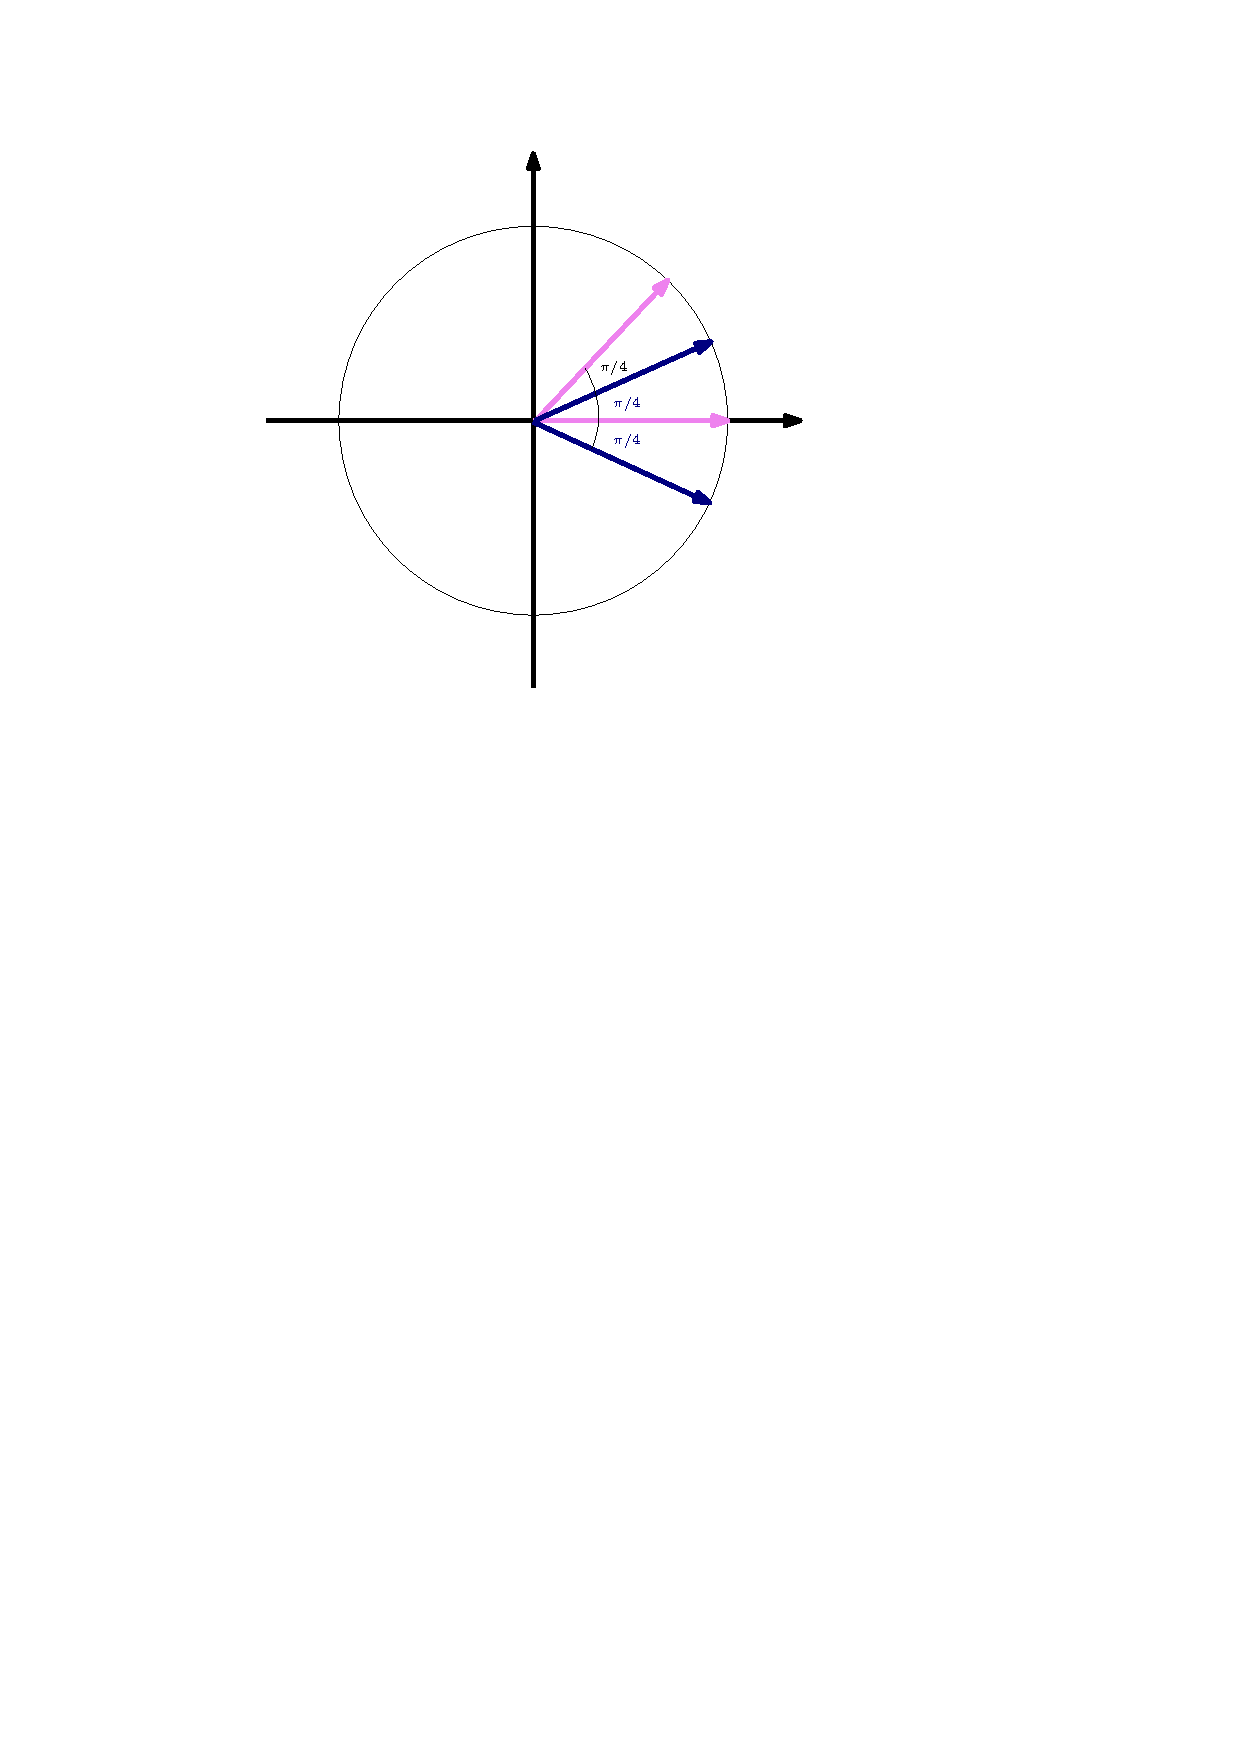
\includegraphics[width=\linewidth]{images/vectors.pdf}

\end{column}
\end{columns}


\end{frame}
\begin{frame}{Uwaga}
    \begin{figure}
        \centering
        
\includegraphics[width=0.5\linewidth]{images/buty.png}
        \label{fig:enter-label}
    \end{figure}
        Istotne jest, że gracze mierzą inne cechy układu (mierzą w innych bazach). Właśnie to daje nam przewagę kwantową.

\end{frame}
\begin{frame}{Związek z nierównością CHSH}
 
Gra CHSH jest równoważna nierówności CHSH. Prawdopodobieństwo wygranej wyraża się wzorem:
\[
  P_{\text{win}} = \frac{S + 4}{8}, \qquad S = 8P_{\text{win}} - 4
\]
gdzie $S = |E(a,b) + E(a,b') + E(a',b) - E(a',b')|$.
 
\medskip
 
\begin{block}{Porównanie granic}
\vspace{-1em}
\begin{center}
\begin{tabular}{lcc}
\toprule
& \textbf{Nierówność CHSH} & \textbf{Gra CHSH} \\
\midrule
Klasyczne & $S \leq 2$ & $P_{\text{win}} \leq \tfrac{3}{4}$ \\[4pt]
Kwantowe (Tsirelson) & $S \leq 2\sqrt{2}$ & $P_{\text{win}} \leq \cos^2\!\tfrac{\pi}{8} \approx 0.854$ \\
\bottomrule
\end{tabular}
\end{center}
\end{block}
 
 
\end{frame}

\section{Section 5}
\input{sections/tirelson}

\section{Section 6}

\begin{frame}{Czemu to takie fajne?}
 
Kwantowa strategia daje przewagę nad klasyczną.\\[1mm]
Oznacza to, że stany kwantowe nie mają ukrytych zmiennych.\\
Mechanika kwantowa nie da się w pełni wyjaśnić lokalnymi, deterministycznymi teoriami.\\[1mm]
\pause
Gra CHSH to eksperymentalna weryfikacja twierdzenia Bella~-- za to przyznano Nagrodę Nobla (2022).\\
 
\pause
 
Zatem Einstein nie miał racji:
\vspace{1em}
\\
\textit{"Bóg nie tylko gra w kości, ale czasem rzuca je tam,
      gdzie ich nie widać."}
 
\hfill\small--- Stephen Hawking
 
\end{frame}
%---------------------------------------------------------
% \begin{frame}{Źródła}
% \label{references}
%     \begin{itemize}
%         \item Marcin Kozik, Anna Szymańska, Andrzej A. Kwaśniewski, \href{https://www.mimuw.edu.pl/~ben/Papers/universes.pdf}{\textit{Płotki małe i duże}}, 2026. \\
%     \end{itemize}

% \end{frame}

%---------------------------------------------------------
\begin{frame}{Źródła}
    \begin{itemize}
        \item \textit{Quantum Information Theory},
        kurs, Universidad Autónoma de Barcelona.\\
        \item M.A. Nielsen, I.L. Chuang,
        \textit{Quantum Computation and Quantum Information},
        Cambridge University Press, 2000.\\
 
        \item IBM Quantum Learning,
        \href{https://quantum.cloud.ibm.com/learning/en/courses/basics-of-quantum-information/entanglement-in-action/chsh-game}{\textit{Basics of Quantum Information: CHSH game}}, 2024.\\

 
        \item J.S. Bell,
        \textit{On the Einstein Podolsky Rosen Paradox},
        Physics, 1(3): 195–200, 1964.\\
 
        \item J.F. Clauser, M.A. Horne, A. Shimony, R.A. Holt,
        \textit{Proposed experiment to test local hidden-variable theories},
        Phys.\ Rev.\ Lett., 23(15): 880–884, 1969.\\
    \end{itemize}
        \begin{tikzpicture}[remember picture,overlay]
        \node[anchor=south east, xshift=-0.2cm, yshift=0.2cm] at (current page.south east)
        {
\includegraphics[width=2cm]{images/martwy_kot.png}};
    \end{tikzpicture}
\end{frame}

\end{document}